\documentclass{beamer}

\mode<presentation>
{
  \setbeamertemplate{navigation symbols}{}
  \setbeamertemplate{caption}[numbered]
  \setbeamertemplate{footline}[frame number]
} 
% \beamertemplatenavigationsymbolsempty

\usepackage[english]{babel}
\usepackage[utf8]{inputenc}
% \usepackage[numbers]{natbib}
\usepackage{natbib}

% \usepackage{lipsum}

\usepackage{mathtext}
\usepackage[T2A]{fontenc}

\setcounter{tocdepth}{1}

\usepackage{amsmath,amssymb}
\usepackage{tikz}
\usetikzlibrary{matrix,positioning,decorations.pathreplacing}


\usepackage{graphicx}
\usepackage{xcolor}
\usepackage{caption}
\usepackage{subcaption}
\usepackage{grffile}

\graphicspath{{../../assets/}}

\newcommand{\real}{\mathbb{R}}
\newcommand{\cplx}{\mathbb{C}}
\newcommand{\conj}[1]{\overline{#1}}
% \newcommand{\iu}{{\imath}}
\newcommand{\iu}{{\jmath}}
% \newcommand{\iu}{{\mathrm{i}}}
% \newcommand{\iu}{{i\mkern1mu}}

\title[Exam]{Bayesian Sparsification of Deep Complex-valued networks}

\author[Nazarov I., Burnaev E.]{Ivan Nazarov, Evgeny Burnaev}

\date{\today}

\institute[Skoltech]{Skolkovo Institute of Science and Technology}

\begin{document}

\begin{frame}[c,plain,noframenumbering]
  \titlepage

\end{frame}

\section{Synopsis} % (fold)
\label{sec:synopsis}

\begin{frame}[c]{\insertsection}
  Motivation for $\cplx$-valued neural networks
  \begin{itemize}
    \item perform better for naturally $\cplx$-valued data
    \item use half as much storage, but the same number of flops
    % \item So inducing sparsity becomes important for lower arithmetic complexity
  \end{itemize}

  \pause
  \medskip
  Propose \emph{Sparse Variational Dropout} for $\cplx$-valued neural networks
  \begin{itemize}
    \item Bayesian sparsification method with $\cplx$-valued distributions 
    % \item $\cplx$-Gaussian variational posterior, $\cplx$-valued priors
    \item empirically explore the compression-performance frontier
  \end{itemize}

  \pause
  \medskip
  Conclusions
  \begin{itemize}
    \item $\cplx$-valued methods compress similarly to the original $\real$ methods
    \item final performance benefits from fine-tuning sparsified network
    \item compress a SOTA $\cplx$VNN on MusicNet by $50-100\times$ at a moderate performance penalty
  \end{itemize}

\end{frame}

% section synopsis (end)

\section{$\cplx$-valued neural networks} % (fold)
\label{sec:complex_valued_networks}

\begin{frame}[c]{\insertsection: Motivation}

  Rectangular form: $z = \Re{z} + \iu \Im{z}$, $\iu^2 = -1$
  \begin{itemize}
    \item $\Re{z}$ and $\Im{z}$ are \textbf{real} and \textbf{imaginary} parts of $z$
  \end{itemize}

  \smallskip
  Polar form: $z = r e^{\iu \phi}$
  \begin{itemize}
    \item $r = \lvert z \rvert$ -- modulus, $\phi = \arg{\!(z)}$ -- argument of $z$
  \end{itemize}

  \pause
  \bigskip
  Benefits of using complex numbers $\cplx$ in neural networks
  \begin{itemize}
    \pause
    \item Richer representation via phase and amplitude $
        r e^{\,\iu \phi} \in \cplx
      $,
      {\tiny \\ \quad
        \citep{reichert_neuronal_2014}}

    \pause
    \smallskip
    \item Non-degenerate combined phase-amplitude transformations,
      {\tiny \\ \quad
        \citep{hirose_generalization_2012}}
    % \item ability to compute multiscale windowed spectra
    %   {\tiny \\ \quad
    %     \citep{bruna_mathematical_2015}}
    % \smallskip

    \pause
    \smallskip
    \item Stable BPTT in RNN via unitary transition matrices,
      {\tiny \\ \quad
        \citep{arjovsky_unitary_2016,wisdom_full-capacity_2016}}
  \end{itemize}

\end{frame}

\begin{frame}[c]{\insertsection: Applications}
%  * applications with 
%  * list of references which consider complex-valued networks and their application and motivation
  Natural $\cplx$-valued data representation
  \begin{itemize}
    \pause
    \item radar and satellite imaging
      {\tiny \\ \quad
        \citep{hirose_complex-valued_2009,hansch_complex-valued_2010,zhang_complex-valued_2017}}

    \smallskip
    \item magnetic resonance imaging
      {\tiny \\ \quad
        \citep{hui_mri_1995,wang_deepcomplexmri_2020}}

    \pause
    \smallskip
    \item radio signal classification
      {\tiny \\ \quad
        \citep{yang_complex_2019,tarver_design_2019}}

    \smallskip
    \item spectral speech modelling and music transcription
      {\tiny \\ \quad
        \citep{wisdom_full-capacity_2016,trabelsi_deep_2018,yang_complex_2019}}
  \end{itemize}
  % \medskip
  % key impediment: what 
  % Timeline
  % % $\cplx$-valued convolutional NN 
  % \citep{hansch_complex-valued_2010} later \citep{popa_complex-valued_2017,zhang_complex-valued_2017}
  % % $\cplx$ RNN with holographic associative memory
  % \citep{danihelka_associative_2016}
  % % unitary transition matrices
  % \citep{wisdom_full-capacity_2016}
  % % $\cplx$-valued Batchnorm and Init
  % \citep{trabelsi_deep_2018}
  % % complex-valued transformer
  % \citet{yang_complex_2019}
  % % quaternion netwroks
  % \citep{gaudet_deep_2018}

  \pause
  \medskip
  Exploring benefits beyond $\cplx$-valued data
  \begin{itemize}
    \item sequence modelling, dynamical system identification
      {\tiny \\ \quad
        \citep{danihelka_associative_2016,wisdom_full-capacity_2016}}

    \smallskip
    \item image classification, road~/~lane segmentation  % KITTI Road Estimation
      {\tiny \\ \quad
        \citep{popa_complex-valued_2017,trabelsi_deep_2018,gaudet_deep_2018}}
  \end{itemize}

\end{frame}

\begin{frame}[c]{\insertsection: Implementation}
  % main reference \citep{trabelsi_deep_2018}, but need some historical perspective
  % $\cplx$VNN operate on complex numbers $\cplx$ instead of real numbers $\real$

  % \medskip
  % \citep{arjovsky_unitary_2016,wisdom_full-capacity_2016,trabelsi_deep_2018,gaudet_deep_2018}
  An intricate double-$\real$ network that respects $\cplx$-arithmetic
  \vspace{-1em}
  \begin{columns}[T]
    \begin{column}{0.45\linewidth}
      \begin{figure}
        % \begin{center}
          % https://tex.stackexchange.com/questions/176432/block-matrix-equation-with-dimensioning

% \documentclass{article}

% \usepackage{tikz}
% \usetikzlibrary{matrix,positioning,decorations.pathreplacing}

% \begin{document}


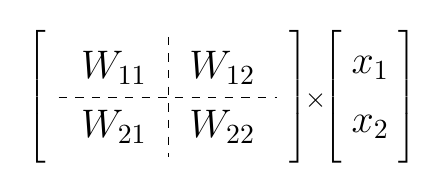
\begin{tikzpicture}[
  style1/.style={
    matrix of math nodes,
    every node/.append style={text width=#1,align=center,minimum height=2.5ex},
    nodes in empty cells,
    left delimiter=[,
    right delimiter=],
    }
  ]
  \matrix[style1=3ex] (1mat)
  {
    & & & \\
    & & & \\
    & & & \\
    & & & \\
  };
  \draw[dashed]
    (1mat-1-2.north east) -- (1mat-4-2.south east);
  \draw[dashed]
    (1mat-2-1.south west) -- (1mat-2-4.south east);
  % \draw[dashed]
  %   (1mat-6-2.south east) -- (1mat-9-2.south east);
  \node[font=\Large]
    at (1mat-1-1.south east) {$W_{11}$};
  \node[font=\Large]
    at (1mat-1-3.south east) {$W_{12}$};
  \node[font=\Large]
    at (1mat-3-1.south east) {$W_{21}$};
  \node[font=\Large]
    at (1mat-3-3.south east) {$W_{22}$};

  \node at ([xshift=2.5ex,yshift=-1.2pt]1mat.east) {$\times$};

  \matrix[style1=1ex,right=5ex of 1mat] (2mat)
  {
    \\
    \\
    \\
    \\
  };
  % \draw[dashed]
  %   (2mat-2-1.south west) -- (2mat-2-1.south east);
  \node[font=\Large] 
    at (2mat-1-1.south) {$x_{1}$};
  \node[font=\Large] 
    at (2mat-3-1.south) {$x_{2}$};
\end{tikzpicture}

% \end{document}

        % \end{center}
        {$\real$VNN linear operation}
        % {$\real$VNN $W x$}
      \end{figure}
    \end{column}%
    \begin{column}{0.45\linewidth}
      \begin{figure}
        % \begin{center}
          % https://tex.stackexchange.com/questions/176432/block-matrix-equation-with-dimensioning

% \documentclass{article}

% \usepackage{tikz}
% \usetikzlibrary{matrix,positioning,decorations.pathreplacing}

% \begin{document}


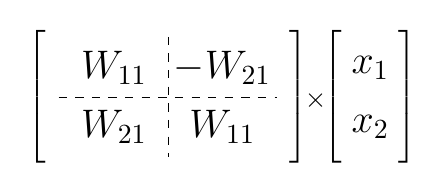
\begin{tikzpicture}[
  style1/.style={
    matrix of math nodes,
    every node/.append style={text width=#1,align=center,minimum height=2.5ex},
    nodes in empty cells,
    left delimiter=[,
    right delimiter=],
    }
  ]
  \matrix[style1=3ex] (1mat)
  {
    & & & \\
    & & & \\
    & & & \\
    & & & \\
  };
  \draw[dashed]
    (1mat-1-2.north east) -- (1mat-4-2.south east);
  \draw[dashed]
    (1mat-2-1.south west) -- (1mat-2-4.south east);
  % \draw[dashed]
  %   (1mat-6-2.south east) -- (1mat-9-2.south east);
  \node[font=\Large]
    at (1mat-1-1.south east) {$W_{11}$};
  \node[font=\Large]
    at (1mat-1-3.south east) {$-W_{21}$};
  \node[font=\Large]
    at (1mat-3-1.south east) {$ W_{21}$};
  \node[font=\Large]
    at (1mat-3-3.south east) {$W_{11}$};

  \node at ([xshift=2.5ex,yshift=-1.2pt]1mat.east) {$\times$};

  \matrix[style1=1ex,right=5ex of 1mat] (2mat)
  {
    \\
    \\
    \\
    \\
  };
  % \draw[dashed]
  %   (2mat-2-1.south west) -- (2mat-2-1.south east);
  \node[font=\Large] 
    at (2mat-1-1.south) {$x_1$};
  \node[font=\Large] 
    at (2mat-3-1.south) {$x_2$};
\end{tikzpicture}

% \end{document}

        % \end{center}
        {$\cplx$VNN linear operation}
        % {$\cplx$VNN $(W_{11} + iW_{21}) (x_1 + i x_2)$ }
      \end{figure}
    \end{column}
  \end{columns}

  \bigskip

  \pause
  \bigskip
  % \item nonlinearities: trigonometric, real-imaginary ReLU etc.
  Activations
  \begin{itemize}
    \item split $
      z \mapsto g(\Re{z}) + \iu g(\Im{z}) % split
    $ or $
      z \mapsto g(\lvert z\rvert) e^{\iu \arg{\!(z)}}
    $ % \citep{trabelsi_deep_2018,hirose_generalization_2012,reichert_neuronal_2014} % relu, tanh, sigmoid

    \item full: trigonometric, holomorphic
  \end{itemize}
  % \citep{hirose_complex-valued_2009}  argues that holomorphy and nondifferentiability are non-issues

  \bigskip

  \pause
  \bigskip
  Geometric representation $\cplx \simeq \real^2$ for backpropagation
  % REWRITE THIS
  \begin{itemize}
    \item Wirtinger derivatives $
        \partial_z
      $ and $
        \partial_{\,\conj{z}}
      $ (independent $z$ and ${\conj{z}}$)

    \item $\nabla_z L \propto \partial_{\,\conj{z}} L(z)$ for $L\colon \cplx^m \to \real$
    % \citep{zimmermann_comparison_2011}
  \end{itemize}
    % \citep{trabelsi_deep_2018}, \citep{arjovsky_unitary_2016}
  % So essentially implementing $\cplx$-valued networks boils down consistently
  % structured $\real$-valued with double the dimensions.

\end{frame}

% section complex_valued_networks (end)

\section{Sparsity and compression} % (fold)
\label{sec:compression}

\begin{frame}[c]{\insertsection}
% Compression is not just making the nets smaller, it is also
% making them use less artihmetic operations, or faster ops
  Improve power, storage or throughput efficiency of deep nets
  \begin{itemize}
    \pause
    \item Knowledge distillation
      {\tiny \\ \quad
        \citep{hinton_distilling_2015,balasubramanian_deep_2016}}

    \smallskip
    \item Network pruning
      {\tiny \\ \quad
        \citep{lecun_optimal_1990,seide_conversational_2011,zhu_prune_2018}}

    \pause
    \smallskip
    \item Low-rank matrix~/~tensor decomposition
      {\tiny \\ \quad
        \citep{denton_exploiting_2014,novikov_tensorizing_2015}}

    \smallskip
    \item Quantization and fixed point arithmetic
      {\tiny \\ \quad
        \citep{courbariaux_training_2015,han_deep_2016,chen_fxpnet_2017}}
  \end{itemize}
% Making them smaller or using faster ops:
% * Knowledge distillation -- creating a smaller replica
% * low-rank approximations -- low-rank structure with efficient mat-vec operations
% * quantization -- dynamic range of floating-points to fixed-points and use fixed range int arithmetic
% * sparsisty -- inducing regularizers (lasso)
% * pruning -- remove insignificant parameters

  \pause
  \bigskip
  Applications to $\cplx$VNN:
  \begin{itemize}
    \item $\cplx$ modulus pruning, quantization with $k$-means in $
        \real^2%\simeq \cplx
      $, 
      {\tiny \\ \quad
        \citep{wu_compressing_2019}}

    \smallskip
    \item $\ell_1$ regularization for hyper-complex-valued networks,
      {\tiny \\ \quad
        \citep{vecchi_compressing_2020}}
      % same calculus relaxation as in $\cplx\real$ calculus
  \end{itemize}

\end{frame}

\subsection{Sparse Variational Dropout} % (fold)
\label{sub:sparse_variational_dropout}

\begin{frame}[c]{\insertsubsection}{\citep{molchanov_variational_2017}}
  % Bayesian perspective on dropout model regularization proposed by Kingma at al. (2015)
  % repurposed for sparsification by Molchanov et al. (2017) and Kharitonov et al. (2018)
  Variational Inference with automatic relevance determination effect
  \begin{equation}
    \label{eq:elbo}
    \underset{
      {\color{orange} q} \in \mathcal{Q}
      % , {\color{teal} \theta}
    }{\text{maximize}}
    \quad
    \underbrace{
      \mathbb{E}_{w \sim {\color{orange} q}}
        % \overbrace{
          \log p(D\mid w)  % ; {\color{teal} \theta})
        % }^{
          % \text{model}
          % \,
          % x\mapsto \hat{y}_w(x)
        % }
    }_{
      \text{data model likelihood}
    }
    \quad
    - \underbrace{
      \mathop{KL}({\color{orange} q}\|{\color{blue} \pi})
    }_{
      \text{variational regularization}
    }
    \tag{ELBO}
  \end{equation}

  % Bayesian inference objective: combine prior assumptions with data into posterior beliefs
  % VI -> SGVB: Jordan (VI), Hoffman (SVI), Kingma (SGVB) (give the elbo equation)
  % Combine prior assumptions with data into posterior beliefs
  \medskip
  prior ${\color{blue} \pi}$
    $\to$ data model likelihood
    $\to$ posterior ${\color{orange} q}$
    (close to $p(w \mid D)$)

  \bigskip

  \pause
  \bigskip
  % Bayesian interpretation of Dropout of \citep{kingma_variational_2015}
  % repurposed for parameter pruning by 
  Factorized Gaussian dropout posterior family $\mathcal{Q}$
  \begin{itemize}
    \item $
      w_{ij} \sim {\color{orange} q}(w_{ij})
        = \mathcal{N}(
          w_{ij}\,\big\vert\,
          {\color{teal} \mu_{ij}},
          {\color{red} \alpha_{ij}}
            {\color{teal} \mu_{ij}}^2
        )
    $, $\alpha_{ij} > 0$, and ${\color{teal} \mu_{ij}} \in \real$
  \end{itemize}

  \pause
  \medskip
  Factorized prior $
    {\color{blue} \pi}(w_{ij})
      \propto \frac1{\lvert w_{ij}\rvert}
  $ (VD)
  \begin{itemize}
    \item (ARD) $
      {\color{blue} \pi}(w_{ij}) = \mathcal{N}(
        w_{ij}\,\big\vert\,
        0, \tfrac1{{\color{teal} \tau_{ij}}}
      )
    $, \citep{kharitonov_variational_2018}
    % precision $\tau_{ij} > 0$
  \end{itemize}

\end{frame}

% subsection sparse_variational_dropout (end)

% section compression (end)

\section{$\cplx$-valued Variational Dropout} % (fold)
\label{sec:extension_to_complex_parameters}

\begin{frame}[c]{\insertsection}{Out proposal}
  \medskip
  % The same objective, but with proper Complex-valued distributions
  Factorized complex-valued posterior $
    {\color{orange} q}(w) = \prod {\color{orange} q}(w_{ij})
  $
  \begin{itemize}
    \item \emph{independent} $
      \mathcal{CN}(
        w_{ij}\,\big\vert\,
        {\color{teal} \mu_{ij}},
        \sigma_{ij}^2,
        \sigma_{ij}^2 \xi_{ij}
      )
    $, $
      \sigma_{ij}^2
        = {\color{red} \alpha_{ij}} \lvert {\color{teal} \mu_{ij}} \rvert^2
    $, $\lvert \xi_{ij} \rvert \leq 1$

    \pause
    \medskip
    \item \emph{circular symmetry} about ${\color{teal} \mu_{ij}}$: fix $
      \xi_{ij} = 0
    $

    % \smallskip
    % \item $
    %   w_{ij} \sim {\color{orange} q}(w_{ij})
    % $ is $
    %   \cplx\mathcal{N}(
    %     {\color{teal} \mu_{ij}},
    %     \sigma^2_{ij},
    %     0
    %   )
    % $ where $
    %   {\color{teal} \mu_{ij}} \in \cplx
    % $ and $
    %   \sigma^2_{ij}
    %     = {\color{red} \alpha_{ij}}
    %       \lvert {\color{teal} \mu_{ij}} \rvert^2
    % $

    \pause
    \medskip
    \item parameter relevance $
      \propto \frac1{{\color{red} \alpha_{ij}}}
    $ and $
      \tfrac{2 \lvert w_{ij} - {\color{teal} \mu_{ij}} \rvert^2}
            {{\color{red} \alpha_{ij}} \lvert {\color{teal} \mu_{ij}} \rvert^2}
    $ is $\chi^2_2$
    % \chi^2_2 is exp(1)
  \end{itemize}

  \bigskip

  \pause
  \bigskip
  \begin{columns}[T]
    \begin{column}{0.60\linewidth}
      Factorized complex-valued priors ${\color{blue} \pi}$
      \begin{itemize}
        \item ($\cplx$-VD) $
          {\color{blue} \pi}(w_{ij})
              \propto \lvert w_{ij}\rvert^{-\rho}
        $, $\rho \geq 1$
        \smallskip
        \item ($\cplx$-ARD) $
          {\color{blue} \pi}(w_{ij})
              = \mathcal{CN}(
                0, \tfrac1{{\color{teal} \tau_{ij}}}, 0
              )
        $
      \end{itemize}
    \end{column}
    \begin{column}{0.30\linewidth}
      \begin{figure}
        \centering
        % 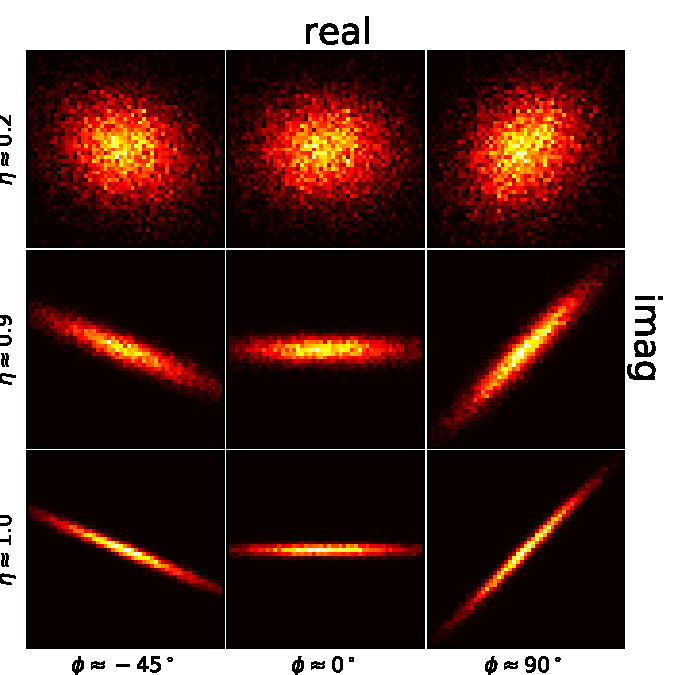
\includegraphics[scale=0.35]{figure__cplx_gaussian.pdf}
        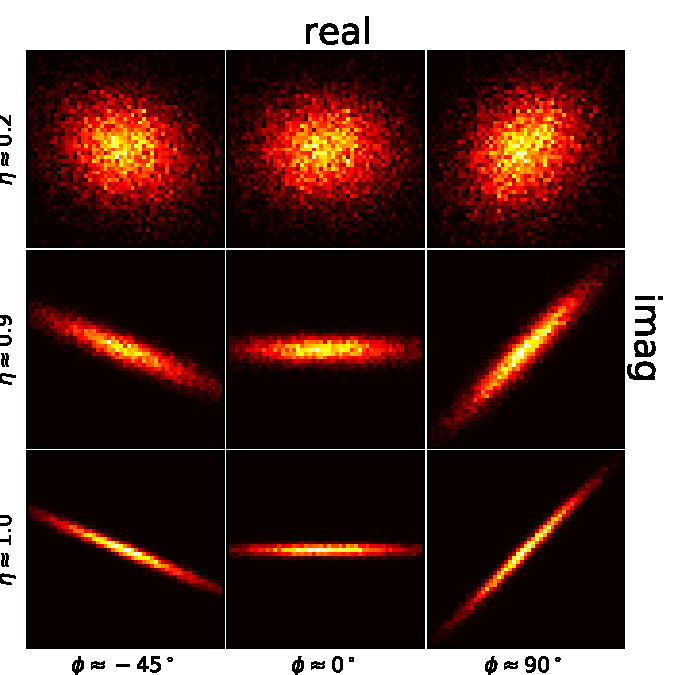
\includegraphics[width=1.2\linewidth]{figure__cplx_gaussian.pdf}
        \quad\mbox{
          \scriptsize
          $\mathcal{CN}(0, 1, \eta e^{\jmath \phi})$, $\lvert \eta \rvert \leq 1$
        }
      \end{figure}
    \end{column}
  \end{columns}

\end{frame}


\begin{frame}[c]{\insertsection}

  $\mathop{KL}({\color{orange} q} \| {\color{blue} \pi})$ term in \eqref{eq:elbo}:
  \begin{equation*}
    \mathop{KL}({\color{orange} q} \| {\color{blue} \pi})
      = \sum_{ij} \mathop{KL}({\color{orange} q}(w_{ij}) \| {\color{blue} \pi}(w_{ij}))
  \end{equation*}

  \pause
  \bigskip
  ($\cplx$-VD) improper prior
  \begin{eqnarray*}
    \mathop{KL}\nolimits_{ij}
      &\propto&
        \tfrac{\rho - 2}2 \log \lvert {\color{teal} \mu_{ij}} \rvert^2
        + \log \tfrac1{{\color{red} \alpha_{ij}}}
        - \tfrac\rho2 Ei( - \tfrac1{{\color{red} \alpha_{ij}}})
      \\
    Ei(x) &=& \int_{-\infty}^x e^t t^{-1} dt
      % \,, \tfrac{d}{dx} Ei(x) = \tfrac{e^x}{x}
  \end{eqnarray*}
  % with $Ei\colon (-\infty, 0) \to \real \colon x \mapsto \int_{-\infty}^x e^t t^{-1} dt$
  % is the exponential integral

  \pause
  \bigskip
  ($\cplx$-ARD) prior is optimized w.r.t. ${\color{teal} \tau_{ij}}$ in empirical Bayes
  \begin{eqnarray*}
    \mathop{KL}\nolimits_{ij}
      &=& -1
        - \log \sigma^2_{ij} {\color{teal} \tau_{ij}}
        + {\color{teal} \tau_{ij}} (\sigma^2_{ij} + \lvert {\color{teal} \mu_{ij}} \rvert^2)
      \\
    \min_{{\color{teal} \tau_{ij}}} \mathop{KL}\nolimits_{ij}
      &=& \log \bigl( 1 + \tfrac1{{\color{red} \alpha_{ij}}} \bigr)
      % \,\text{ at }
      % {\color{teal} \tau_{ij}}
      %   = (\sigma^2_{ij} + \lvert {\color{teal} \mu_{ij}} \rvert^2)^{-1}
  \end{eqnarray*}

\end{frame}

% subsection _cplx_valued_gaussian_distribution (end)

% section extension_to_complex_parameters (end)

\section{Experiments} % (fold)
\label{sec:experiments}

\begin{frame}[t]{\insertsection}{Datasets}
  Four MNIST-like datasets
  % MNIST, Fashion-MNIST, KMNIST, EMNIST-Letters
  \begin{itemize}
    % \item channel features ($\real \hookrightarrow \cplx$ with $\Im z = 0$) or $2$d Fourier features
    \item channel features ($\real \hookrightarrow \cplx$) or $2$d Fourier features
    \item fixed random subset of $10k$ train samples
    \item simple dense and convolutional nets
  \end{itemize}
  % do not train to convergence, just show that the methods give comparable results under similar conditions

  \pause
  \medskip
  CIFAR10 dataset ($\real^3 \hookrightarrow \cplx^3$)
  \begin{itemize}
    \item random cropping and horizontal flipping
    \item $\cplx$-valued variant of VGG16 {\tiny \citep{simonyan_very_2015}}
  \end{itemize}

  \pause
  \medskip
  Music transcription on MusicNet {\tiny \citep{thickstun_learning_2017}}
  \begin{itemize}
    \item audio dataset of $330$ annotated musical compositions
    \item use power spectrum to tell which piano keys are pressed
    \item deep $\cplx$VNN proposed by \citep{trabelsi_deep_2018}
  \end{itemize}

\end{frame}

\begin{frame}[c]{\insertsection}{Set-up}
  % methodological contrib
  $\beta$-VAE \ref{eq:elbo} objective {\tiny \citep{higgins_beta-vae_2017}}
  \begin{equation}
  \label{eq:beta_elbo}
    \max_q
    \mathbb{E}_{w \sim {\color{orange} q}}
      \log p(y\mid w, x)  % ; {\color{teal} \theta})
    - \beta \mathop{KL}({\color{orange} q}\|{\color{blue} \pi})
    \tag{$\beta$-ELBO}
  \end{equation}
  \vspace{-1em}
  \begin{itemize}
    \item balance the likelihood and prior-matching terms' feedback
    \item explore performance-compression trade-off by varying $\beta$
    % \item KL-div annealing of \citet{molchanov_variational_2017} does not allow
    % to explore the performance-compression trade-off
  \end{itemize}

  \pause
  \medskip
  % methodological contrib
  Three-stage training:
  \begin{enumerate}
    \item `pre-train' the network as-is with deterministic layers
    \item `compress' with $\real$/$\cplx$-Variational Dropout layers
    \item `fine-tune' pruned network (relevant parameters only)
    % sparse layers are sloooow
  \end{enumerate}

  \pause
  \medskip
  Pruning based on estimated ${\color{red} \alpha_{ij}}$ and threshold
  \begin{itemize}
    \item $
      \log{{\color{red} \alpha_{ij}}} \leq -\tfrac12
    $ ensures that $
      w_{ij} \sim {\color{orange} q}(w_{ij})
    $ concentrates around ${\color{teal} \mu_{ij}}$
    % \item Relevant $w_{ij}$ are concentrated around ${\color{teal} \mu_{ij}}$ w.h.p according ${\color{orange} q}$
    % \item \citet{molchanov_variational_2017} use $\tau=3$, tied to Bernoulli Dropout with rate $95\%$
  \end{itemize}
  % A picture of the typical $\log \alpha$ distribution? bimodal

\end{frame}

% section experiments (end)

\section{Results} % (fold)
\label{sec:results}

\begin{frame}[c]{\insertsection}{MNIST}
  \begin{figure}[t]
    \begin{subfigure}[b]{0.5\columnwidth}
      \centering
      % 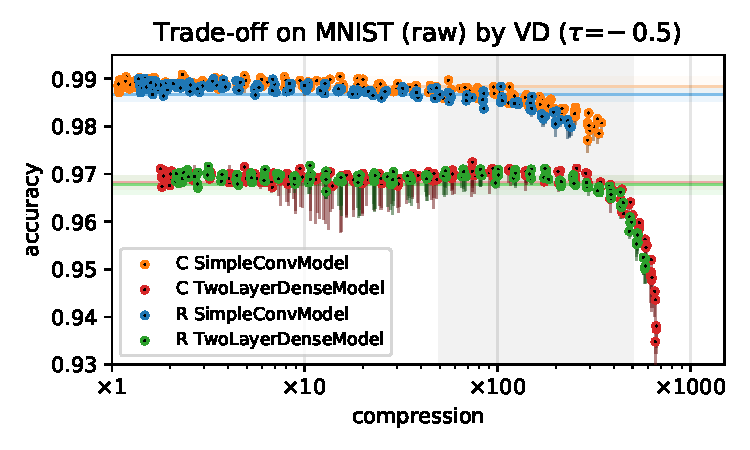
\includegraphics[width=\linewidth]{figure__mnist-like__trade-off/appendix__VD__mnist__raw__-0.5.pdf}
      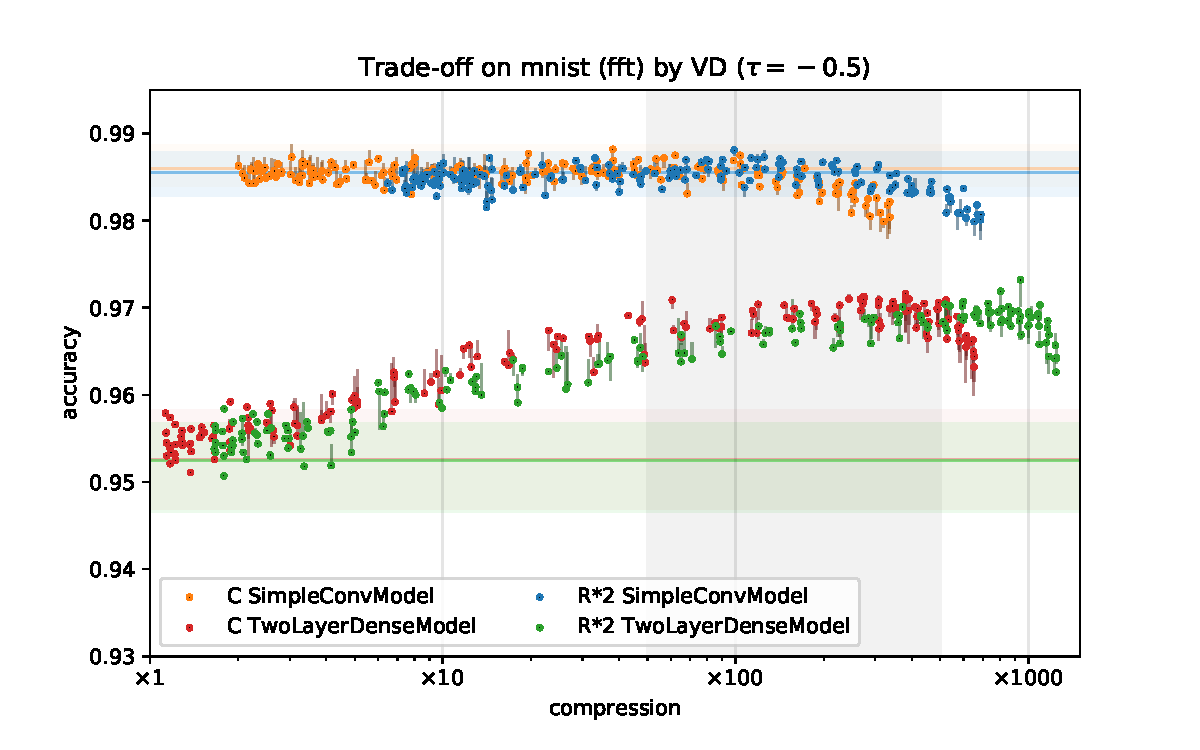
\includegraphics[width=\linewidth]{figure__mnist-like__trade-off/appendix__cmp__VD__mnist__fft__-0.5.pdf}
    \end{subfigure}\hspace{-1em}%
    \begin{subfigure}[b]{0.5\columnwidth}
      \centering
      % 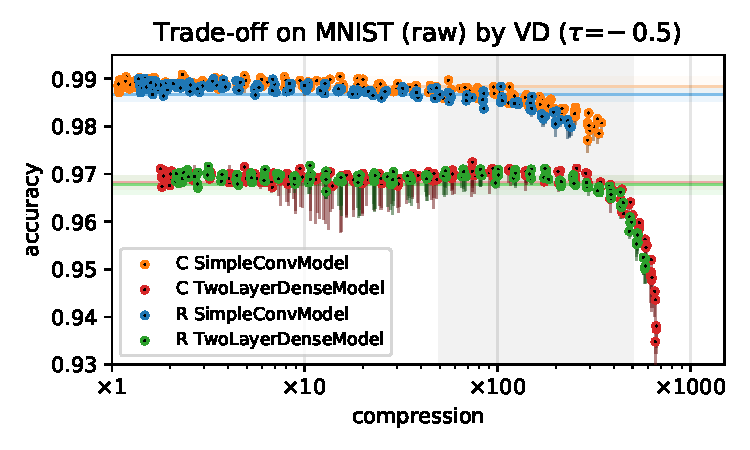
\includegraphics[width=\linewidth]{figure__mnist-like__trade-off/appendix__VD__mnist__raw__-0.5.pdf}
      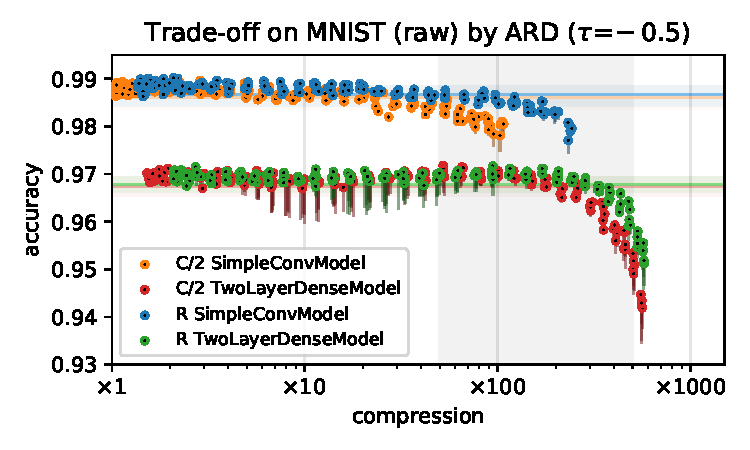
\includegraphics[width=\linewidth]{figure__mnist-like__trade-off/appendix__cmp__ARD__mnist__raw__-0.5.pdf}
    \end{subfigure} \\ %
    \begin{subfigure}[b]{0.5\columnwidth}
      \centering
      % 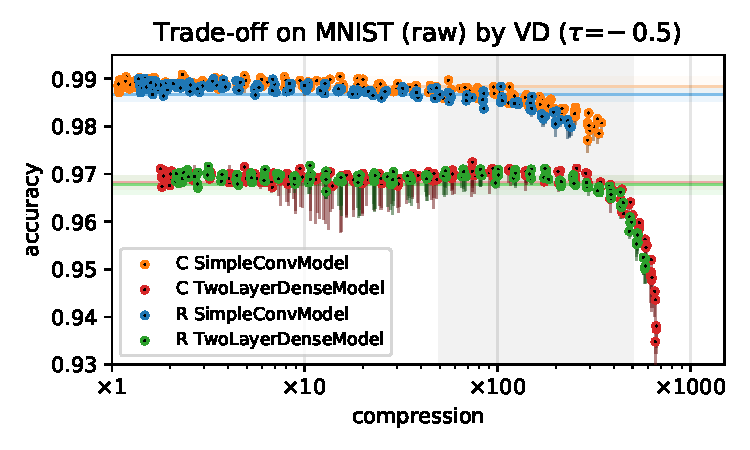
\includegraphics[width=\linewidth]{figure__mnist-like__trade-off/appendix__VD__mnist__raw__-0.5.pdf}
      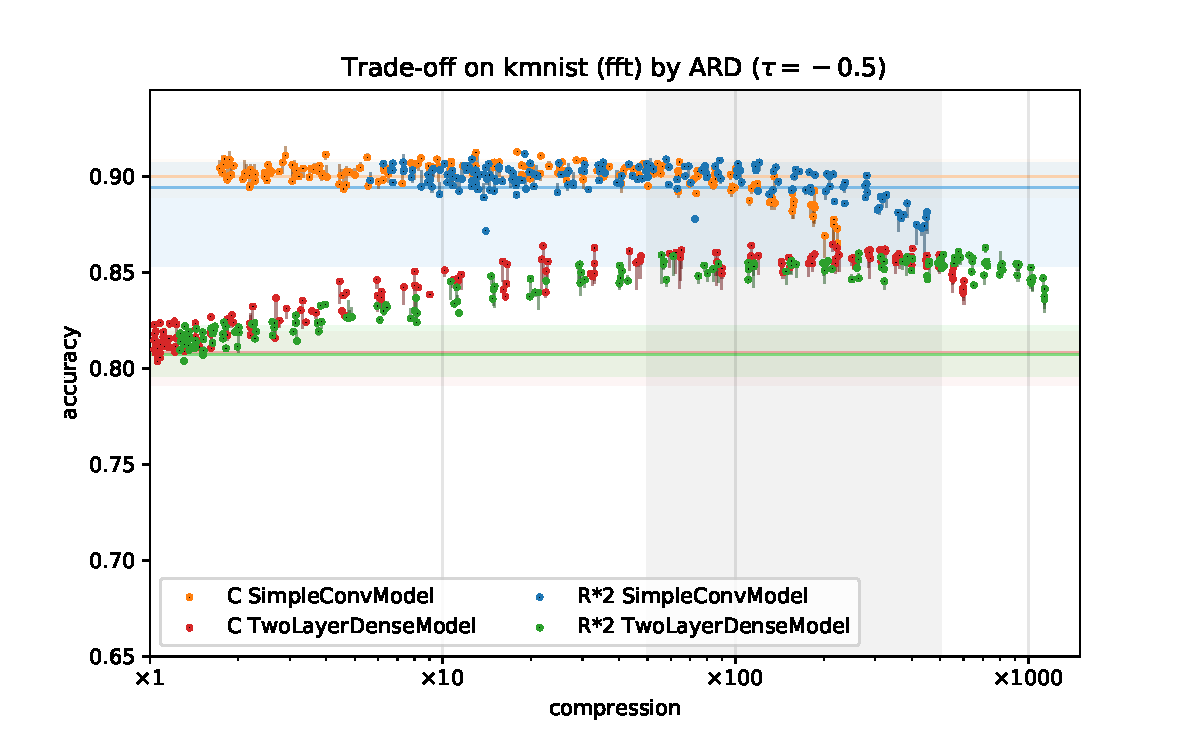
\includegraphics[width=\linewidth]{figure__mnist-like__trade-off/appendix__cmp__ARD__kmnist__fft__-0.5.pdf}
    \end{subfigure}\hspace{-1em}%
    \begin{subfigure}[b]{0.5\columnwidth}
      \centering
      % 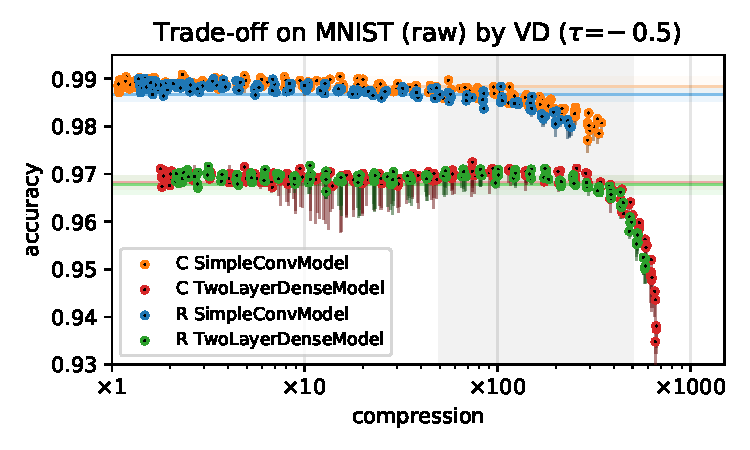
\includegraphics[width=\linewidth]{figure__mnist-like__trade-off/appendix__VD__mnist__raw__-0.5.pdf}
      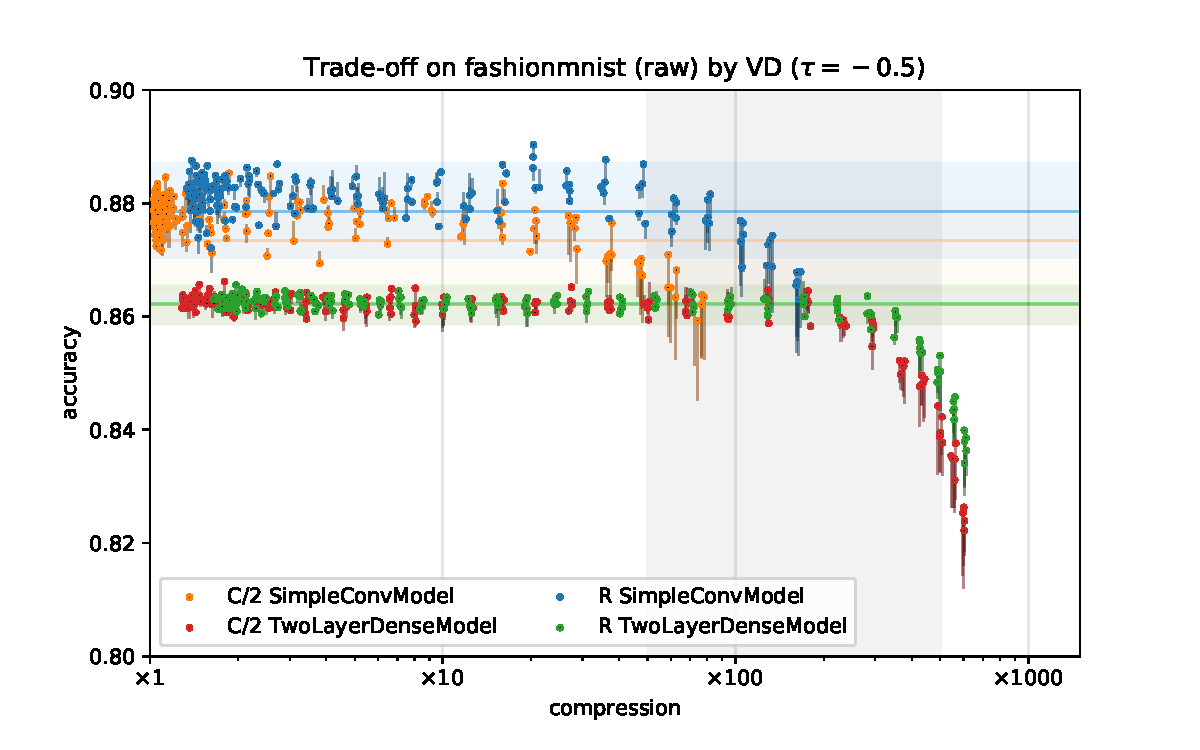
\includegraphics[width=\linewidth]{figure__mnist-like__trade-off/appendix__cmp__VD__fashionmnist__raw__-0.5.pdf}
    \end{subfigure}%
  \end{figure}

\end{frame}

\begin{frame}[c]{\insertsection}{CIFAR10}
  \begin{figure}[t]
    \centering
    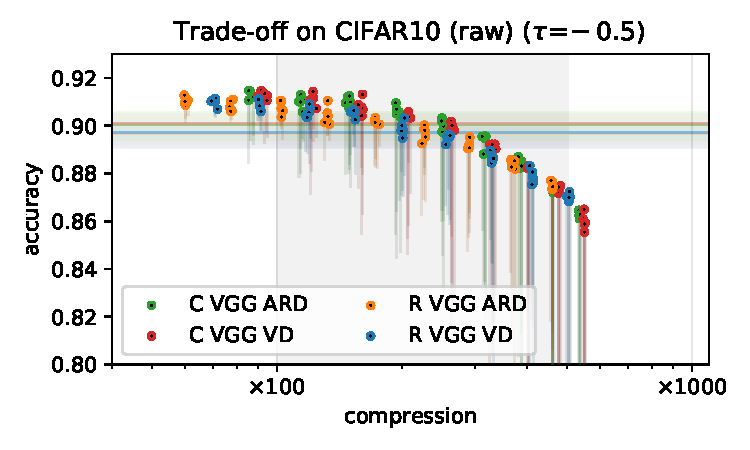
\includegraphics[width=\linewidth]{figure__cifar__trade-off/appendix__augmentedcifar10__raw__-0.5.pdf}
    \\
    {$\cplx$-valued version of VGG16 \citep{simonyan_very_2015}}
  \end{figure}

\end{frame}

\begin{frame}[c]{\insertsection}{MusicNet}
  \begin{figure}[t]
    \centering
    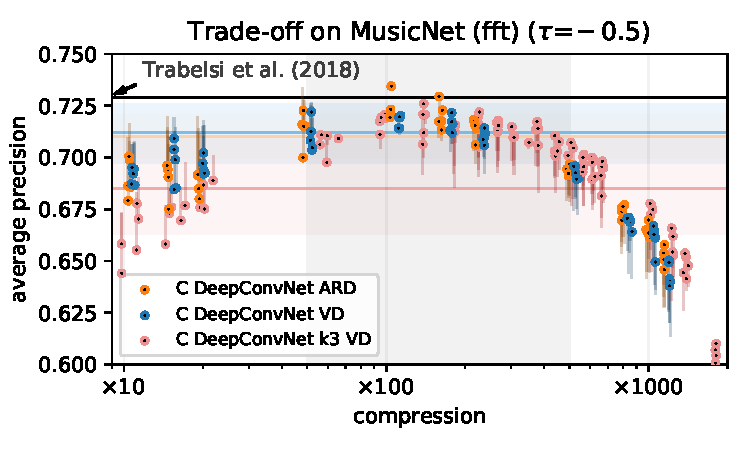
\includegraphics[width=\linewidth]{figure__musicnet__trade-off/paper__musicnetram__fft__-0.5.pdf}
    \\
    {The $\cplx$VNN of \citet{trabelsi_deep_2018}}
  \end{figure}

  % \pause
  % \medskip
  % \begin{enumerate}
  %   \item $77.3\%$ four-layer $\real$-network, $\log$-spaced STFT features
  %     % with cosince window to prevent spectral leakeage
  %     {\tiny \\ \citet{thickstun_invariances_2018}}
  %   \item $74.2\%$ $\cplx$-transformer
  %     {\tiny \\ \citet{yang_complex_2019}}
  %   \item $72.9\%$ VGG-like $\cplx$-net
  %     {\tiny \\ \citet{trabelsi_deep_2018}}
  % \end{enumerate}

\end{frame}

\begin{frame}[c]{\insertsection}{Effects of $\tau$}
  \begin{figure}[t]
    \centering
    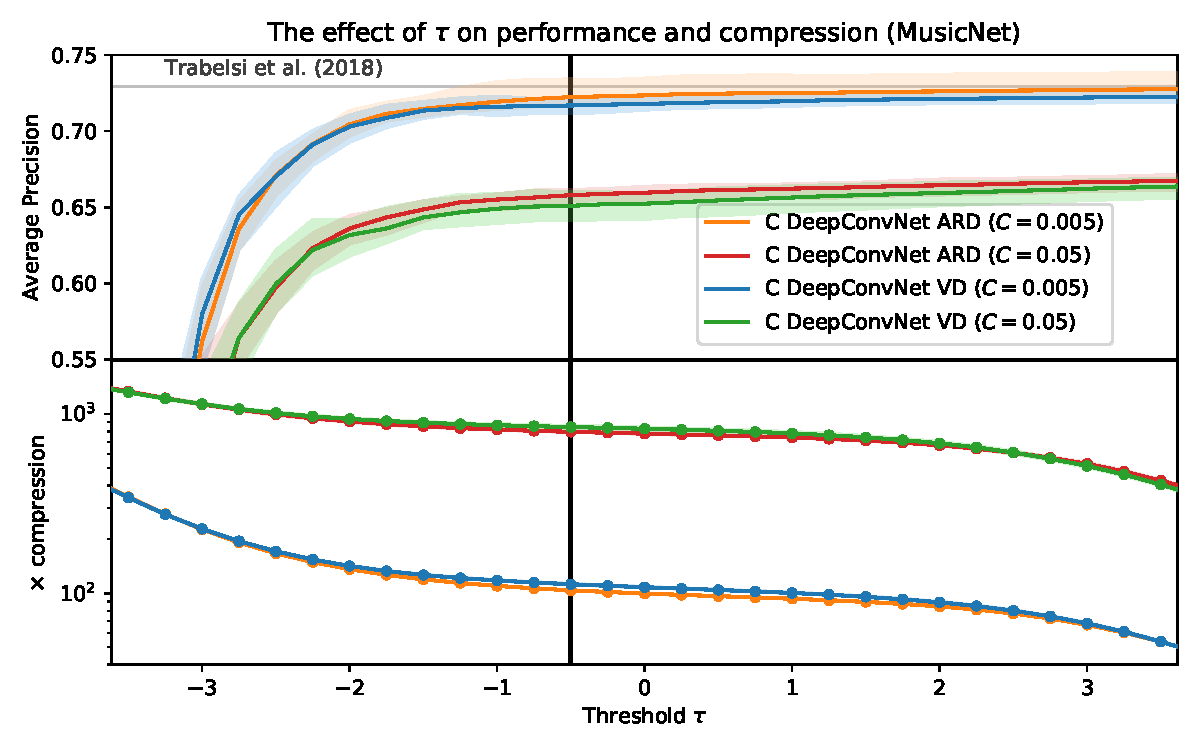
\includegraphics[width=\linewidth]{figure__musicnet__threshold.pdf}
    \\
    {Before `fine-tune' of the $\cplx$VNN of \citet{trabelsi_deep_2018}}
  \end{figure}

\end{frame}

\begin{frame}[c]{Effects of $\tau$}{\insertsection}
  \begin{figure}[t]
    \centering
    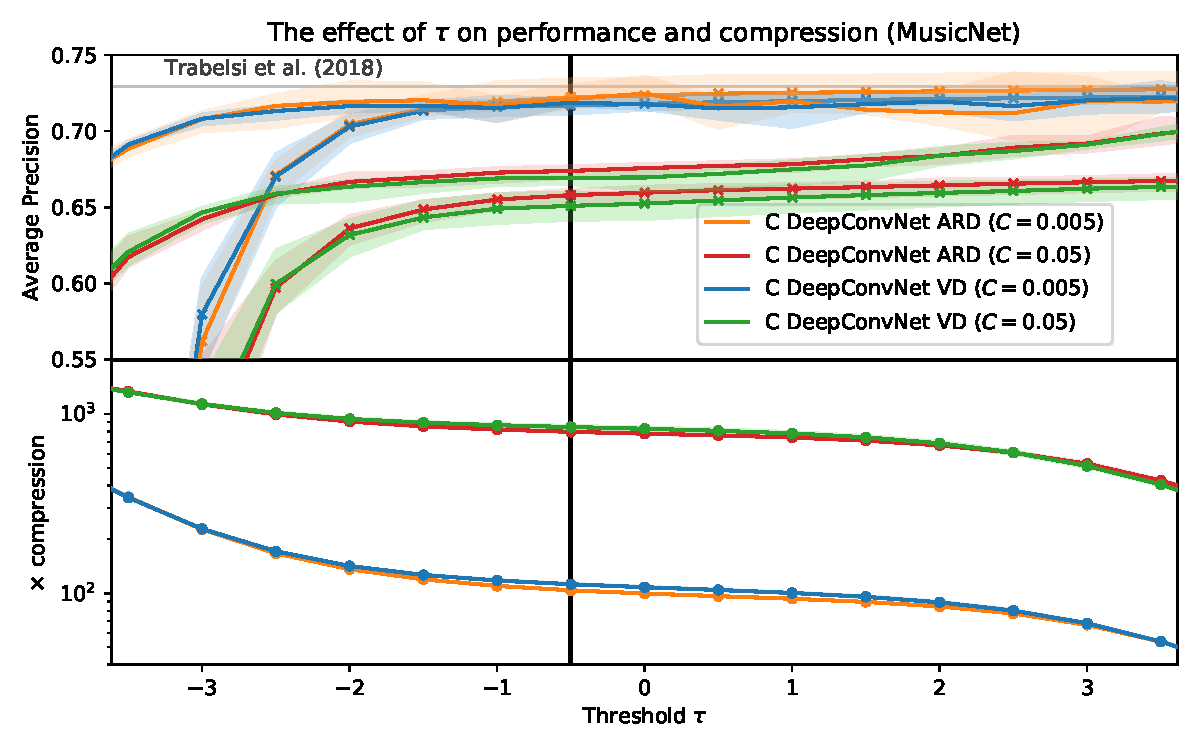
\includegraphics[width=\linewidth]{figure__musicnet__threshold__fine-tune.pdf}
    \\
    {After `fine-tune' of the $\cplx$VNN of \citet{trabelsi_deep_2018}}
  \end{figure}

\end{frame}

% section results (end)

\section{Summary} % (fold)
\label{sec:summary}

\subsection{Results} % (fold)
\label{sub:results}

\begin{frame}[c]{\insertsubsection}{\insertsection}
  % Recap
  Bayesian sparsification of $\cplx$-valued networks
  \begin{itemize}
    \item proposed $\cplx$-VD and $\cplx$-ARD methods
    \item investigated performance-compression trade-off
    \item compress the $\cplx$VNN of \citet{trabelsi_deep_2018}
    by $50-100\times$ at a small performance penalty
  \end{itemize}

  \pause
  \medskip
  Experiments
  \begin{itemize}
    \item $\cplx$-VD and $\cplx$-ARD have trade-off similar to $\real$ methods
    % no clear winner across replications and datasets in terms of compression and performance
    \smallskip
    \item $\real$-networks tend to compress better than $\cplx$-nets
    \smallskip
    \item fine-tuning improves performance in high compression regime
    % in line with prior lit \citep{han_learning_2015}
    % \item Variational Dropout controllably removes redundancy in wide $\cplx$ and $\real$ networks
    \smallskip
    \item weak effect on performance~/~compression than $\beta$ in \eqref{eq:beta_elbo}
    % \item compression results are replicable and stable
  \end{itemize}

  % \pause
  % \medskip
  % Conclusions of \citep{gale_state_2019} should carry over to $\cplx$VNN
  % \begin{itemize}
  %   \item $\ell_0$ regularization uses multiplicative hard-concrete mask
  %     {\tiny \\ \citep{louizos_learning_2018}}
  %   \item pruning relies on absolute-value rankings
  %     {\tiny \\ \citep{zhu_prune_2018}}
  % \end{itemize}
  % % Fourier features on images do not provide advantages

\end{frame}

% subsection results (end)

\subsection{Limitations} % (fold)
\label{sec:limitations}

\begin{frame}[c]{\insertsubsection}{\insertsection}

  \emph{Circular symmetry} of the posterior ${\color{orange} q}(w_{ij})$ about
  ${\color{teal} \mu_{ij}}$ implies \emph{independence} of $\Re$ and $\Im$
  % var fmaily based on cgauss implies independence
  % * if we use this param then can model polarization
  \begin{itemize}
    \item richer variational approximation family
    \item $\cplx$-ARD ${\color{blue} \pi}$ and learn relation $
      \xi = {\color{teal} \eta} e^{\iu {\color{teal} \phi}}
    $ in ${\color{orange} q}$
  \end{itemize}

  \bigskip

  \pause
  \bigskip
  \emph{Factorized} ${\color{orange} q}$ implies parameter independence % in ${\color{orange} q}$ does not hold in practice
  \begin{itemize}
    \item structured sparsity is desirable for fast computations and hardware implementations
    % \item structured sparsity is desirable for SIMD-processing
    % \item parameter coupling may give higher compression, \citep{citation_needed}
  \end{itemize}

\end{frame}

% subsection limitations (end)

% section summary (end)

\section{References} % (fold)
\label{sec:references}

\begin{frame}<beamer:0>[t,noframenumbering,plain,allowframebreaks]{\insertsection}
  \tiny
  \bibliographystyle{abbrvnat}
  \bibliography{presentation}
\end{frame}

% section references (end)

\appendix
\begin{frame}[c]{MusicNet}{\insertsection}
  Poor performance of under-compressed $\cplx$VNN of \citet{trabelsi_deep_2018}
  \begin{itemize}
    \item `pre-train' validation score peaks at $\approx 15$ epochs
    \item `fine-tune' essentially continues `pre-train' for small $\beta$ in \eqref{eq:beta_elbo}
  \end{itemize}

  \begin{figure}[t]
    \centering
    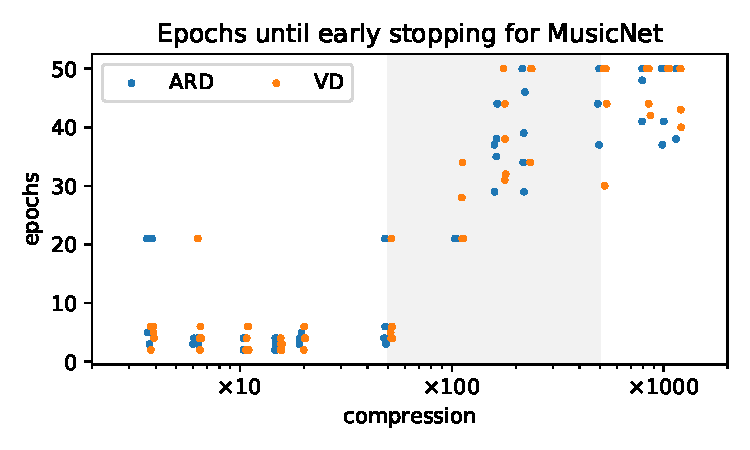
\includegraphics[width=\linewidth]{figure__fine-tune_fx__early__compression.pdf}
  \end{figure}
\end{frame}

\end{document}
